%!TEX program = xelatex

% \documentclass[10pt]{article}
%%%%%%%%%%%%%%%%%%%%%%%%%%%%%%%%%%%%%%%%%
% Modified By Orcuslc, 2016-9-12
% http://github.com/orcuslc
%
% Wilson Resume/CV
% Structure Specification File
% Version 1.0 (22/1/2015)
%
% This file has been downloaded from:
% http://www.LaTeXTemplates.com
%
% License:
% CC BY-NC-SA 3.0 (http://creativecommons.org/licenses/by-nc-sa/3.0/)
%
%%%%%%%%%%%%%%%%%%%%%%%%%%%%%%%%%%%%%%%%%

%----------------------------------------------------------------------------------------
%	PACKAGES AND OTHER DOCUMENT CONFIGURATIONS
%----------------------------------------------------------------------------------------

\usepackage[a4paper, hmargin=25mm, vmargin=30mm, top=20mm]{geometry} % Use A4 paper and set margins

\usepackage{fancyhdr} % Customize the header and footer

\usepackage{lastpage} % Required for calculating the number of pages in the document

\usepackage{hyperref} % Colors for links, text and headings

\setcounter{secnumdepth}{0} % Suppress section numbering

%\usepackage[proportional,scaled=1.064]{erewhon} % Use the Erewhon font
%\usepackage[erewhon,vvarbb,bigdelims]{newtxmath} % Use the Erewhon font
\usepackage[utf8]{inputenc} % Required for inputting international characters
\usepackage[T1]{fontenc} % Output font encoding for international characters

\usepackage{fontspec} % Required for specification of custom fonts
\setmainfont[Path = ./fonts/,
Extension = .otf,
BoldFont = Erewhon-Bold,
ItalicFont = Erewhon-Italic,
BoldItalicFont = Erewhon-BoldItalic,
SmallCapsFeatures = {Letters = SmallCaps}
]{Erewhon-Regular}

\usepackage{color} % Required for custom colors
\definecolor{slateblue}{rgb}{0.17,0.22,0.34}

\usepackage{sectsty} % Allows customization of titles
\sectionfont{\color{slateblue}} % Color section titles

\fancypagestyle{plain}{\fancyhf{}\cfoot{\thepage\ of \pageref{LastPage}}} % Define a custom page style
\pagestyle{plain} % Use the custom page style through the document
\renewcommand{\headrulewidth}{0pt} % Disable the default header rule
\renewcommand{\footrulewidth}{0pt} % Disable the default footer rule

\setlength\parindent{0pt} % Stop paragraph indentation

% Non-indenting itemize
\newenvironment{itemize-noindent}
{\setlength{\leftmargini}{0em}\begin{itemize}}
{\end{itemize}}

% Text width for tabbing environments
\newlength{\smallertextwidth}
\setlength{\smallertextwidth}{\textwidth}
\addtolength{\smallertextwidth}{-2cm}

\newcommand{\sqbullet}{~\vrule height 1ex width .8ex depth -.2ex} % Custom square bullet point definition

%----------------------------------------------------------------------------------------
%	MAIN HEADER COMMAND
%----------------------------------------------------------------------------------------

\renewcommand{\title}[1]{
{\huge{\color{slateblue}\textbf{#1}}}\\ % Header section name and color
\rule{\textwidth}{0.5mm}\\ % Rule under the header
}

%----------------------------------------------------------------------------------------
%	JOB COMMAND: Modified by Orcuslc 2016-09-12
%----------------------------------------------------------------------------------------

\newcommand{\job}[6]{
\begin{tabbing}
\hspace{2cm} \= \kill
\textbf{#1} \> \href{#4}{\textbf{#3}} \\
\textbf{#2} \>\+ \textit{#5} \\
\begin{minipage}{\smallertextwidth}
\vspace{2mm}
#6
\end{minipage}
\end{tabbing}
\vspace{2mm}
}

%----------------------------------------------------------------------------------------
%	SKILL GROUP COMMAND - Modified by Orcuslc 2016-09-12
%----------------------------------------------------------------------------------------

\newcommand{\skillgroup}[2]{
% \begin{tabbing}
% \hspace{5mm} \= \kill
% \sqbullet \> \textbf{#1}
% \end{tabbing}
% \begin{tabbing}
% \vspace{-2pt}
% \hspace{3cm} \= \kill
% #2
% \end{tabbing}
% }
\begin{tabbing}
\hspace{5mm} \= \kill
\sqbullet \>\+ \textbf{#1} \\

\begin{minipage}{\smallertextwidth}
\vspace{2mm}
#2
\end{minipage}
\end{tabbing}
}

\newcommand{\skill}[2]{
\begin{tabbing}
\hspace{1cm} \> \hspace{3cm} \= \kill
\>\textbf{#1:} \> #2 \\
\end{tabbing}
% \hspace
}

%----------------------------------------------------------------------------------------
%	INTERESTS GROUP COMMAND
%-----------------------------------------------------------------------------------------

\newcommand{\interestsgroup}[1]{
\begin{tabbing}
\hspace{5mm} \= \kill
#1
\end{tabbing}
\vspace{-10mm}
}

\newcommand{\interest}[1]{\sqbullet \> \textbf{#1}\\[3pt]} % Define a custom command for individual interests


%---------------------------------------------------------------
%   AWARDS GROUP COMMAND: Created by Orcuslc 2016-09-12
%---------------------------------------------------------------
\newcommand{\awardgroup}[1]{
\begin{tabbing}
\hspace{5mm} \= \kill
#1
\end{tabbing}
\vspace{2mm}
}

\newcommand{\award}[2]{
% \begin{tabbing}
% \hspace{0} \> \hspace{2cm} \= \kill
\hspace{2cm} \> \hspace{2cm} \= \kill
\sqbullet \> \textbf{#1} \> #2 \\[3pt]
% \hspace{2cm} \= \kill
% \end{tabbing}

}

%----------------------------------------------------------------------------------------
%	TABBED BLOCK COMMAND: Modified by Orcuslc 2016-09-12
%----------------------------------------------------------------------------------------

\newcommand{\tabbedblock}[1]{
\begin{tabbing}
\hspace{2cm} \= \hspace{4cm} \= \hspace{4cm} \= \hspace{4cm} \= \kill
#1
\end{tabbing}
}

%-----------------------------------------------------------------
%  TABBED BLOCK 2 COMMAND: Created by Orcuslc 2016-09-12
%-----------------------------------------------------------------
\newcommand{\tabblock}[5]{
\begin{tabbing}
% \hspace{2cm} \= \kill
\hspace{2cm} \= \hspace{4cm} \= \hspace{4cm} \= \hspace{4cm} \= \kill

\textbf{#1} \> \textbf{#3} \\
\textbf{#2} \> \textbf{#4} \\[5pt]
\>\+
#5
\end{tabbing}
}


%-----------------------------------------------------------------
%  RESEARCH COMMAND: Created by Orcuslc 2016-09-12
%-----------------------------------------------------------------
\newcommand{\research}[7]{
\begin{tabbing}
\hspace{2cm} \= \kill
\textbf{#1} \> \textbf{#3}, under the supervision of \href{#5}{\textbf{#4}} \\
% \href{#4}{#3} \\
\textbf{#2} \>\+ \textit{#6} \\
\begin{minipage}{\smallertextwidth}
\vspace{0.5mm}
#7
\end{minipage}
\end{tabbing}
\vspace{2mm}
}

%-------------------------------------------------------------------------
%      Programming Projects Command - Created by Orcuslc 2016-9-14
%-------------------------------------------------------------------------
% \newcommand{\projectgroup}[1]{
% \begin{tabbing}
% % \hspace{5mm} \= \kill
% \vspace{5mm}
% #1
% \end{tabbing}
% }

\newcommand{\projectgroup}[1]{
% \begin{tabbing}
\hspace{5mm} \= \kill
#1
% \end{tabbing}
\vspace{2mm}
}


\newcommand{\project}[3]{
% \begin{tabbing}
\hspace{2cm} \> \hspace{2cm} \= \kill
\sqbullet \> \textbf{#1} \> #2 \\
\> \textbf{code:} \> \href{#3}{#3} \\[5pt]
% \end{tabbing}
}
\usepackage{epstopdf}
\usepackage{graphics}
\usepackage{subfig}
\usepackage{listings}
\lstset{
  numbers=left,
    framexleftmargin=10mm,
    frame=none,
    backgroundcolor=\color[RGB]{245,245,244},
  keywordstyle=\bf\color{blue},
  identifierstyle=\bf,
  numberstyle=\color[RGB]{0,192,192},
  commentstyle=\it\color[RGB]{0,96,96},
  stringstyle=\rmfamily\slshape\color[RGB]{128,0,0},
  showstringspaces=false,
  extendedchars=false
    }
\DeclareGraphicsExtensions{.eps,.ps,.jpg,.bmp}

\begin{document}

\title{Assignment 8}{17.5.6}

\problem{1}{Explain that when $c(x) < 0$, the extremum principle may not stand.}
\solution{Proof}{
Consider the 1-dimension Helmholtz equation:
$$
\frac{d^2u}{dx^2}+k^2u = 1, \quad u(0) = u(1) = 0.
$$
We can find the solution of this equation has a form like
$$
u(x) = \frac{\cos k+1}{k^2\sin k}\cos kx-\frac{1}{k^2}\sin kx+\frac{1}{k^2}.
$$
If we let $k = \frac{\pi}{2}$, then $u'(\frac{1}{2}) = 0$, but $u(\frac{1}{2}) = \frac{4(1-\sqrt{2})}{\pi^2} < 0$. So this time the extremum principle does not stand.
}

\problem{2}{If $u(0) = u(1) = 0$, and $\frac{d^2u}{dx^2} = f(x)$. Prove
$$
u(x) = \int_0^1 G(x; x_0)f(x_0) dx_0
$$
with Green function.}
\solution{Proof}{
In fact, we just check if $u(x)$ satisfies the conditions in the problem. \\
First,
\begin{equation}
\begin{split}
&u(0) = \int_0^1 x_0\times0\times f(x_0)dx_0 = 0, \\
&u(1) = \int_0^1 x_0\times0\times f(x_0)dx_0 = 0.
\end{split}
\end{equation}
Second,
\begin{equation}
\begin{split}
u'(x) &= \int_0^x (1-x_0)f(x_0)dx_0 + (1-x)xf(x) + \int_x^1-x_0f(x_0)dx_0-x(1-x)f(x) \\
&= \int_0^x f(x_0)dx_0-\int_0^1x_0f(x_0)dx_0,
\end{split}
\end{equation}
So $u''(x) = f(x)$, with uniqueness of Cauchy problem, we can prove the $u(x)$ is the function we need.
}

\problem{3}{Consider the equation
$$
-a\frac{d^2u}{dx^2}+b\frac{du}{dx}+cu=1,
$$
with boundary conditions $u(0) = 0$, $\frac{du}{dx}(1)+u(1)=0$, and parameters $a > 0, c\geqslant 0$ in $(0, 1)$. Solve the equation in accurate form and by difference scheme.
}
\solution{Accurate}{
The characteristic equation of this differential equation is 
$$
-a\lambda^2+b\lambda+c = 0.
$$
Case 1: $b = c = 0$. In this case, $u(x) = \frac{-x^2+2}{2a}.$ \\
Case 2: $c = 0, b \ne 0.$ The roots of the characteristic equation are $x_1 = 0, x_2 = -\frac{a}{b}.$ So the general solution is $u(x) = k_1e^{bx/a}+k_2$ for the homogeneous problem. And a special solution of the nonhomogeneous problem is $u = \frac{x}{b}$, and the accurate solution is 
$$
u(x) = -\frac{a}{b^2}e^{bx/a} - \frac{1}{b}e^{b/a} + \frac{x}{b}- \frac{a}{b^2}.
$$
considering the boundary conditions. \\
Case 3: $b, c\ne 0.$ Using the same techniques, the accurate solution is
$$
u(x) = \frac{e^{\lambda_2}-(1+\lambda_1)}{c((1+\lambda_2)e^{\lambda_1}-(1+\lambda_1)e^{\lambda_2})}e^{\lambda_1x} + \frac{e^{\lambda_1}-(1+\lambda_2)}{c((1+\lambda_1)e^{\lambda_2}-(1+\lambda_2)e^{\lambda_1})}e^{\lambda_2x}+\frac{1}{c},
$$
in which $\lambda_1, \lambda_2$ are roots of $-a\lambda^2+b\lambda+c=0$.
}

\solution{Numerical}{
The computing scheme of this problem is
\begin{equation}
-a\frac{u_{i+1}-2u_i+u_{i-1}}{h^2}+b\frac{u_{i+1}-u_{i-1}}{2h}+cu_i = f_i, \quad i = 1, 2, \cdots, N-1.
\end{equation}
Then the linear equation can be written as
$$
\mathbf{Au}+\mathbf{Bu}+\mathbf{Cu} = \mathbf{f},
$$
with
$$
\mathbf{A} = \mathrm{tridiag}(1, -2, 1),
$$
$$
\mathbf{B} = \mathrm{tridiag}(-1, 0, 1),
$$
$$
\mathbf{C} = \mathrm{diag}(1),
$$
$$
\mathbf{f}=\left(                 
  \begin{array}{cccccc}   
    1\\  
    1\\  
    ...\\
    ...\\
    1\\
    1\\
    \end{array}
\right)+\left(                 
  \begin{array}{cccccc}   
    \frac{a}{h^{2}}u_{0}-\frac{b}{2h}u_{0}\\  
    0\\  
    ...\\
    ...\\
    0\\
    \frac{a}{h^{2}}u_{N}-\frac{b}{2h}u_{N}\\
    \end{array}
\right).
$$
We can simply give the solution by
$$
\mathbf{u} = (\mathbf{A+B+C})^{-1}\mathbf{f}.
$$
The numerical simulation is as follows, in which we choose $a = 1, b = 10, c = 10.$
\begin{figure}[!h] \centering
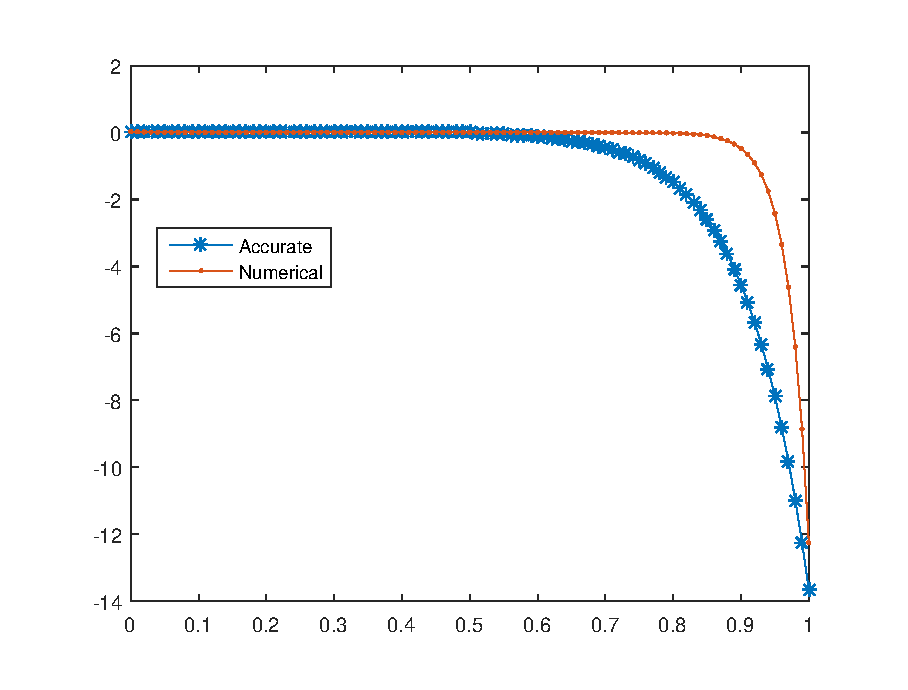
\includegraphics[width = 15cm]{code/Simulation.eps}
\caption{Simulation and Accurate results}
\end{figure}
Relative error is as follows:
\begin{figure}[!h] \centering
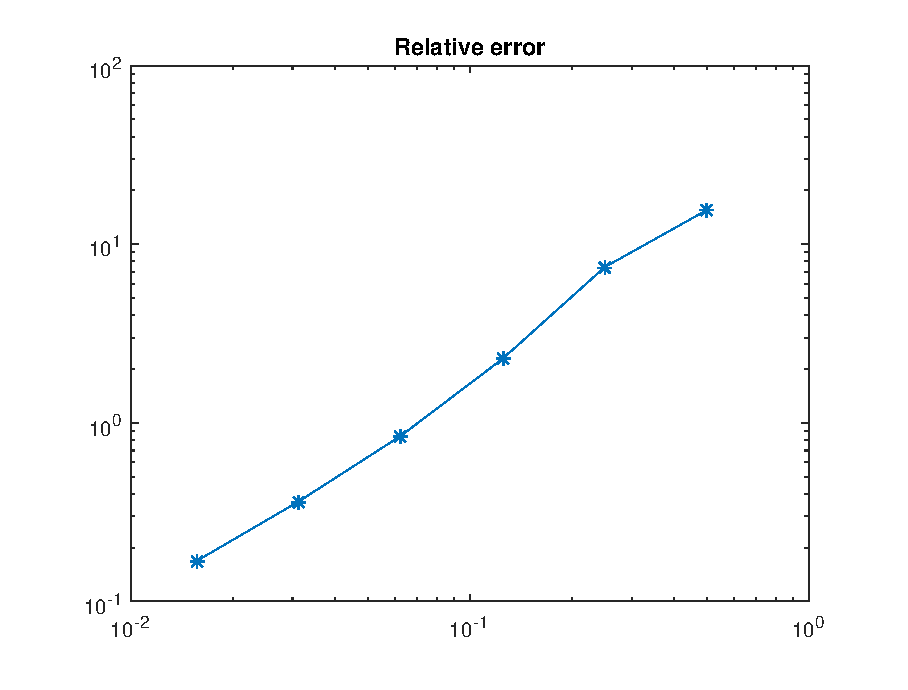
\includegraphics[width = 15cm]{code/error.eps}
\caption{Relative error}
\end{figure}
}


\end{document}